%

\section{Experiments}\label{sec:experiments}

The theoretical guarantees of the previous section demonstrate that common \fielddefnames{} such as \shap{} and \intgradshort{} cannot reliably infer \countmodbehaviourname{}. 
While our assumptions are satisfied by moderately rich \modelname{} classes (including neural networks), 
%
our theory does not rule out the possibility that additional structure extracted from the training data or learning algorithm %
is further aiding \fielddefnames{} in practice.
In this section, we provide experimental results consistent with what our theory predicts, even when we restrict consideration to neural networks trained with stochastic gradient descent on real datasets.
%
%
Specifically, for ReLU neural networks on tabular data and convolutional neural networks on image data, we observe that \shap{} and \intgradshort{} are close to random guessing for the \downtasknames{} of algorithmic recourse and spurious \covname{} identification.
We also compare with three common local methods: gradients, \smoothgrad{}, and \lime{}. 
We find that for simple tabular data, these methods can outperform \shap{} and \intgradshort{}, while for image data all methods are comparable to random guessing.
%
All code is available at \url{https://github.com/google-research/interpretability-theory}.

\subsection{Methods}

To visualize \specname{} and \sensname{}, we use the standard receiver operating characteristic (ROC) curve, which shows the trade-off of the false positive rate (1 -- \specname{}) on the $x$-axis and the true positive rate (\sensname{}) on the $y$-axis. An ROC curve is computed by varying the rejection threshold for a \hyptestname{}: the more strict the threshold, the less likely to reject the null, and hence the lower the false positive rate. An ideal hypothesis test threshold achieves the top left corner of the plot (0\% false positives and 100\% true positives), and generally a hypothesis test is better if the curve is closer to the top left corner of the plot. The diagonal line from $(0,0)$ to $(1,1)$ is the line \specname{} = 1 -- \sensname{}, and hence corresponds exactly to random guessing.

For each dataset, \fielddefname{}, and \downtaskname{}, we construct an empirical ROC curve.
To do so, for each dataset we retrain 10 neural networks (\modelnames{}) using different random seeds to similar accuracy. Then, we randomly sample 20 \obsnames{} from the test dataset and compute each \fielddefname{} on each \obsname{} for each \modelname{}. For each non-categorical \covname{} and each \downtaskname{}, we compute a \hyptestname{} at a specific threshold using the \covname{} \attname{} and compare it to a ``\groundname{}''; for details on the \hyptestnames{} and the \groundname{}, see \cref{sec:examples-tasks}.
Thus, each point on a plot corresponds to a single dataset, \modelname{}, \fielddefname{}, \downtaskname{}, and \hyptestname{} threshold, and represents the empirical true and false positive rates for a \hyptestname{} averaged over all \covnames{} on 20 \obsnames{}.
We repeat each of these calculations with 40 different \hyptestname{} thresholds to create the entire ROC curve.
Since we reuse the same 20 \obsnames{} for each \modelname{}, the noisy ROC curve is actually comprised of 10 different (one for each \modelname{}) monotonic ROC curves.

For image data, it is ambiguous what constitutes a ``\covname{}''. Following the literature \citep{molnar2022}, we consider each individual pixel to be a \covname{}. For computational reasons, we did not average over every pixel for each \hyptestname{}, but instead over a sample of 10 pixels (this matches that most of the tabular datasets have roughly 10 \covnames{}). 
%
%
%

%
%
%
%
%
%
%

%
%

\subsubsection{\downtaskNAMEs{}}\label{sec:examples-tasks}
%
\paragraph{\groundNAME{}}
For both \downtasknames{}, the \groundname{} relies on a neighbourhood around \obsnames{}. For each \obsname{} $\covval$ and \covname{} $j$ we consider, we construct this neighbourhood as follows. We fix a percentage $p \in [0,1]$, and compute a range $R$ which is the maximum value of the $j$th \covname{} minus the minimum value of the $j$th \covname{} on the dataset under consideration. We then create 20 copies of $\covval$, where all \covname{} values are fixed except for the $j$th, which is set to $\covvaldum_j = \covval_j + \delta$ for $\delta$ evenly spaced in $(-pR, pR)$. We display results for $p=0.1$, but found similar results for $p$ ranging from $0.5$ to $0.01$. For smaller $p$, we encountered floating point issues (the model output didn't change at all over the neighbourhood).

\textbf{Recourse.} 
We use the \taskname{} of %
\cref{defn:recourse} for a single \covname{}, with $\covdistdum$ taken to be the uniform distribution.
To compute the \groundname{}, we approximate expectation under this distribution by comparing the empirical average \modelname{} output on the first half of the perturbed \obsnames{} to the empirical average \modelname{} output on the second half of the perturbed \obsnames{}.
That is, the \groundname{} is 1 if the average \modelname{} output is larger from increasing the \covname{} versus decreasing it, and 0 otherwise.

To conduct the \hyptestname{}, we use the sign and magnitude of the \covname{} \attname{}.
In particular, for threshold $\threshval\in\Reals$ and \covname{} \attname{} $\expval\in\Reals$, we use $\oraclehyptest(\expval) = \ind{\expval > \threshval}$.
%
This hypothesis test is consistent with applications in the literature: \citet{aditya20biased} use \shap{} (also accounting for magnitude) and \citet{ghosh22fair} use \intgradshort{} to identify which \covnames{} should be adjusted for to achieve outcome fairness.
%

\textbf{Spurious \covNames{}.} 
%
We use a variant of the  \taskname{} of \cref{defn:spurious}, replacing $\sup$ with variance for better stability.
First, we compute the perturbation described above for 100 additional \obsnames{} from the dataset of interest and then compute the variance of the \modelname{} output over each perturbation (providing an empirical distribution of such variances). 
We then set the $\outscale$ in \cref{defn:spurious} to be the 80th quantile of this empirical distribution, and the \groundname{} is computed by comparing the \modelname{} output variance over the perturbations of the \obsname{} at hand with this $\outscale$. 
That is, the \groundname{} is 1 if perturbing the \covname{} causes the \modelname{} output to vary more than 80\% of other \covnames{}, and 0 otherwise.

To conduct the \hyptestname{}, we use only the magnitude of the \covname{} \attname{}.
In particular, for threshold $\threshval\in\Reals$ and \covname{} \attname{} $\expval\in\Reals$, we use $\oraclehyptest(\expval) = \ind{\abs{\expval} > \threshval}$.

%
%
%
%
%
%
%

%
%
%

\subsubsection{\fielddefNAMEs{}}

\textbf{\shap{}.} For tabular data (i.e., a small number of \covnames{}), we compute \shap{} according to \cref{def:genshap} using the \texttt{KernelExplainer} function from the Python \texttt{shap} package \citep{lundberg17shapley}. We approximate the outer expectation (with respect to the training data distribution) using an empirical average over 100 samples and the inner expectation (with respect to the Shapley kernel over subsets) using an empirical average over 500 samples. For image data, the number of subsets of pixels is too large to approximate accurately, so we follow the \texttt{shap} documentation and use the \texttt{Explainer} function with \texttt{maskers.Image}. This approximates the \shap{} value by ``blocking out'' groups of pixels.

\textbf{\vanillagrad{}.} We compute $\grad \model$ exactly using \texttt{TensorFlow} \citep{tensorflow2015-whitepaper}.

\textbf{\intgrad{}.} We use \cref{def:intgrad}, approximating the integral using a sum with 20 steps. Following \citet{sundararajan17integrated}, we use a pointmass \basename{}, so the expectation does not need to be approximated. 
We visualize two baselines: all \covnames{} set to zero (the mean of the data after rescaling), and all \covnames{} set to their minimum value.

\textbf{\smoothgrad{}.} We use \cref{def:smoothgrad}, where for each $\covval$ we take $\covdist$ to be $\normaldist(\covval, 0.1 \cdot I_\covdim)$ following \citet{smilkov17smoothgrad}. We approximate this expectation using 100 samples.

\textbf{\lime{}.} We use \cref{def:lime}, following the use of the best (regularized) local linear model from \citet{ribeiro16lime}. For simplicity, we set $\lambda = 1$ and for each $\covval$ take $\covdist$ to be $\normaldist(\covval, 0.1 \cdot I_\covdim)$---in \citet{ribeiro16lime}, $\covdist$ is denoted by $\pi_\covval$. We then approximate the expectation using 100 samples so that the $\argmin$ can be found exactly using the closed-form solution of regularized least squares.



\subsubsection{Datasets}

\textbf{Tabular data.} We consider 5 standard tabular datasets from the UCI repository \citep{Dua19UCI}: wine origin (\texttt{wine}) \citep{forina86wine}, credit approval  (\texttt{credit}) \citep{quinlan1987credit}, chess outcome (\texttt{chess}) \citep{bain1994chess}, E.~coli protein localization (\texttt{ecoli}) \citep{nakai1991ecoli}, and abalone age (\texttt{abalone}) \citep{nash1994abalone}. After centering and normalizing the \covnames{} by their empirical standard deviation, we trained small ReLU neural networks on the first four datasets to average test accuracies of 100\%, 80\%, 99\%, and 85\% respectively, while for the \texttt{abalone} dataset (which has integer responses) we achieved average test mean squared error of 4.5.

\textbf{Image data.} We consider 3 standard image datasets: MNIST digit classification (\texttt{mnist}) \citep{lecun2010mnist}, Fashion-MNIST classification (\texttt{fashion}) \citep{xiao17fashion}, and CIFAR-10 image classification (\texttt{cifar-10}) \citep{Krizhevsky09learningmultiple}.
After normalizing the pixel values to $[0,1]$, we trained standard convolutional neural networks to average test accuracies of 99\%, 90\%, and 80\% respectively.


%
%
%
%
%
%
%

%
%
%
%
%
%
%
%
%
%
%
%

%
%

%




\subsection{Results}

We plot ROC curves for all \downtasknames{}, datasets, and attribution methods in \cref{fig:10percent-plots-1} (tabular datasets) and \cref{fig:10percent-plots-2} (image datasets).
We highlight some observations:

\textbf{Observation 1:}
\shap{} and \intgrad{} ROC curves are near random guessing for almost all experiments. This agrees with what our theory suggests.

\textbf{Observation 2:}
The \basename{} for \intgradshort{} matters.
Using a \basename{} of all zeroes is, in general, worse than using a \basename{} corresponding to the minimum \covnames{}.
This difference is to be expected: the choice of \basename{} is already empirically known to heavily influence the output \citep{sturmfels2020visualizing}.
However, we emphasize that (a) both \basenames{} are often near the random guessing line, and (b) \emph{without strong additional knowledge about the dataset and learned \modelname{}, there is no way to know in advance what the ``right'' \basename{} is to choose for your \taskname{}}.

\textbf{Observation 3:}
Simpler, local \fielddefnames{} sometimes outperform \shap{} and \intgradshort{}.  
For some tasks, gradients, \smoothgrad{}, and \lime{} perform much better than random guessing, likely because algorithmic recourse and spurious \covname{} identification are local \downtasknames{}.
These methods are not foolproof, however; for many cases they also fail to improve on random guessing.
Once again, \emph{there is no way to know in advance whether your \fielddefname{} will work for your \taskname{} without strong additional knowledge}.

\textbf{Observation 4:}
The ROC curves suggest that, in general, the end-tasks are easier to solve on tabular datasets than image datasets. 
While for tabular datasets we see many ROC curves far from random guessing, the ROC curves for image datasets are near the diagonal that corresponds to random guessing. 
We conjecture that this is because the \modelnames{} learned for tabular datasets can be quite simple, making gradients (and their variants) more indicative of \countmodbehaviourname{}. (Recall that if the \modelname{} is linear, \countmodbehaviourname{} is recovered exactly by all \methodnames{}.)

\clearpage
\begin{figure*}[!hpt]
\centering
\begin{subfigure}
    \centering
    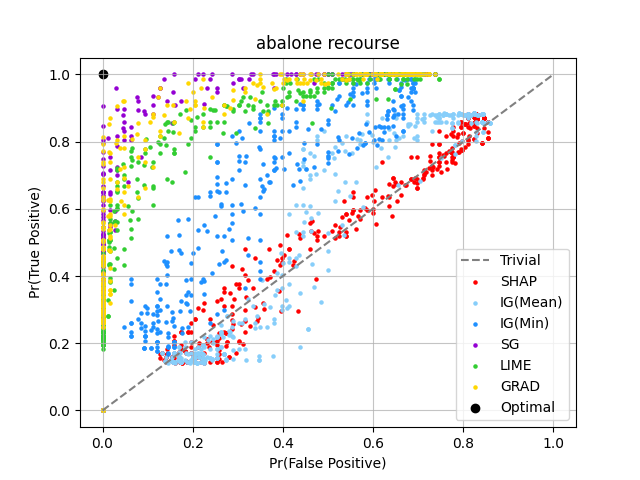
\includegraphics[width=.33\linewidth]{figure-files/experiments/10percent-plots/abalone-recourse-hypothesis-tradeoff.png}
\end{subfigure}
\begin{subfigure}
    \centering
    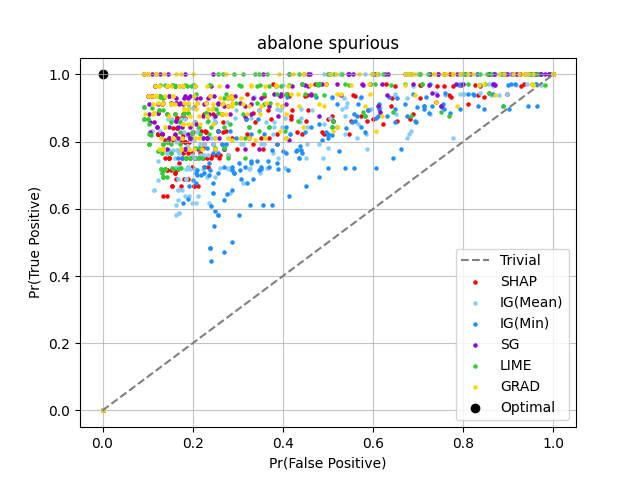
\includegraphics[width=.33\linewidth]{figure-files/experiments/10percent-plots/abalone-spurious-hypothesis-tradeoff.png}
\end{subfigure}
%
\begin{subfigure}
    \centering
    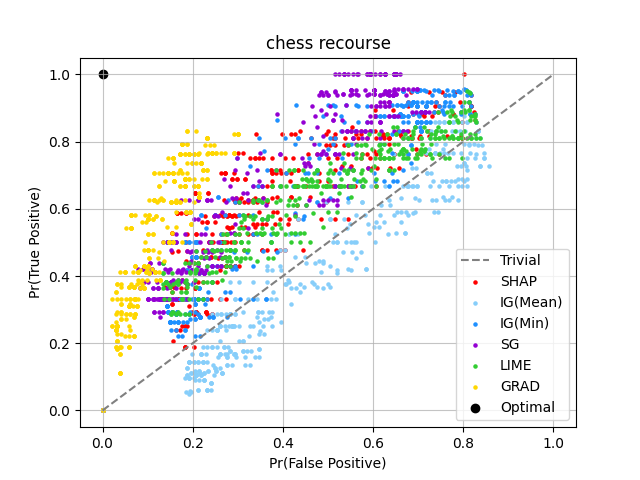
\includegraphics[width=.33\linewidth]{figure-files/experiments/10percent-plots/chess-recourse-hypothesis-tradeoff.png}
\end{subfigure}
\begin{subfigure}
    \centering
    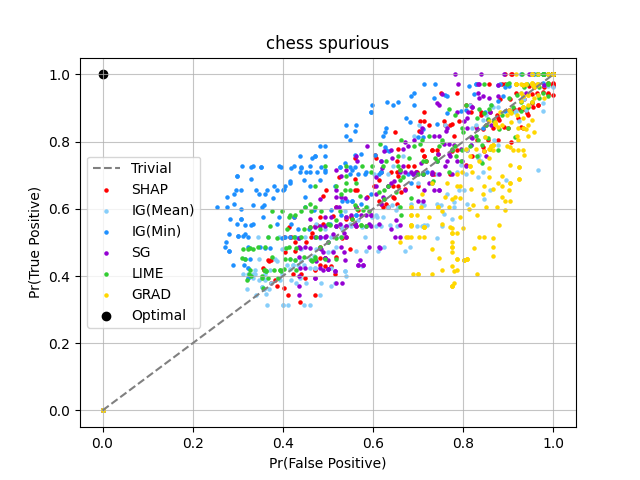
\includegraphics[width=.33\linewidth]{figure-files/experiments/10percent-plots/chess-spurious-hypothesis-tradeoff.png}
\end{subfigure}
%
\begin{subfigure}
    \centering
    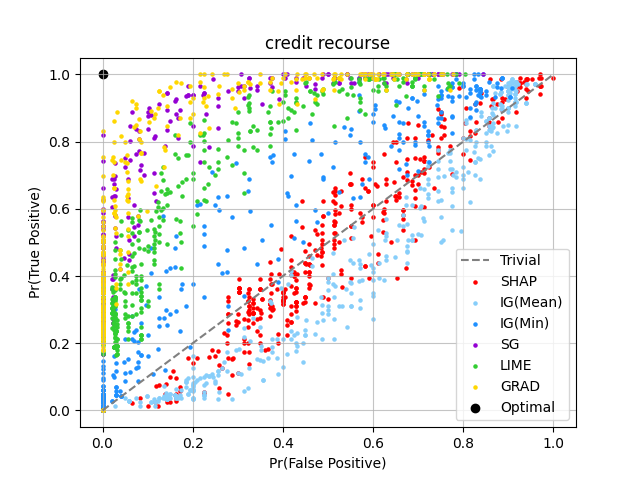
\includegraphics[width=.33\linewidth]{figure-files/experiments/10percent-plots/credit-recourse-hypothesis-tradeoff.png}
\end{subfigure}
\begin{subfigure}
    \centering
    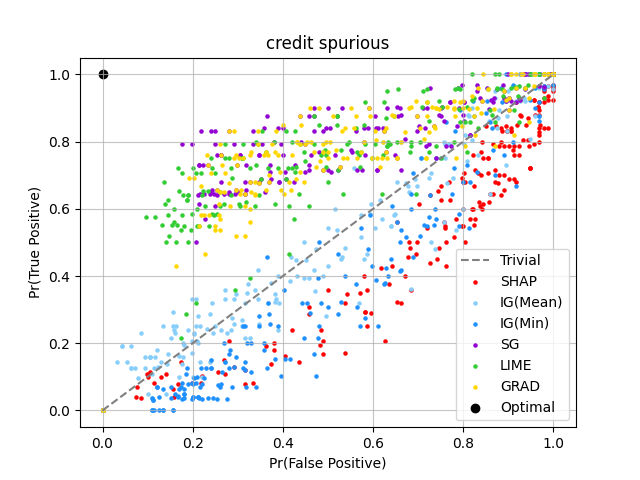
\includegraphics[width=.33\linewidth]{figure-files/experiments/10percent-plots/credit-spurious-hypothesis-tradeoff.png}
\end{subfigure}
%
\begin{subfigure}
    \centering
    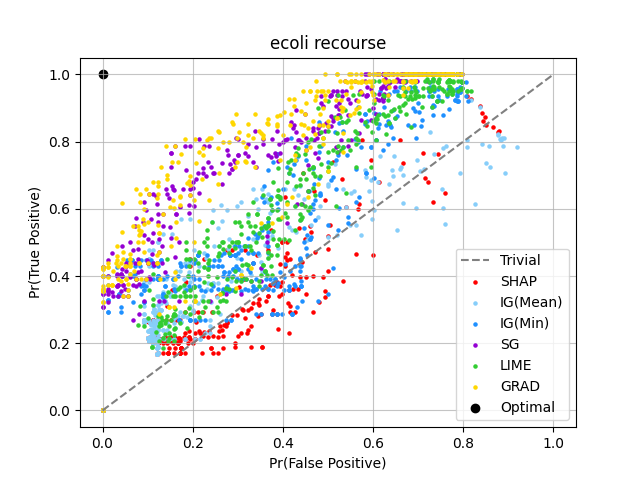
\includegraphics[width=.33\linewidth]{figure-files/experiments/10percent-plots/ecoli-recourse-hypothesis-tradeoff.png}
\end{subfigure}
\begin{subfigure}
    \centering
    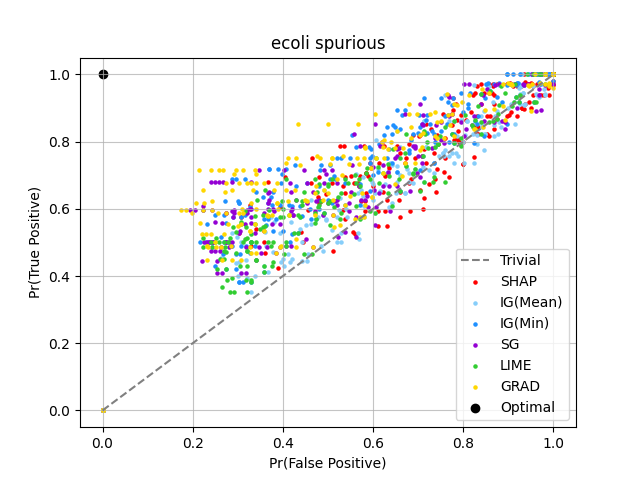
\includegraphics[width=.33\linewidth]{figure-files/experiments/10percent-plots/ecoli-spurious-hypothesis-tradeoff.png}
\end{subfigure}
\begin{subfigure}
    \centering
    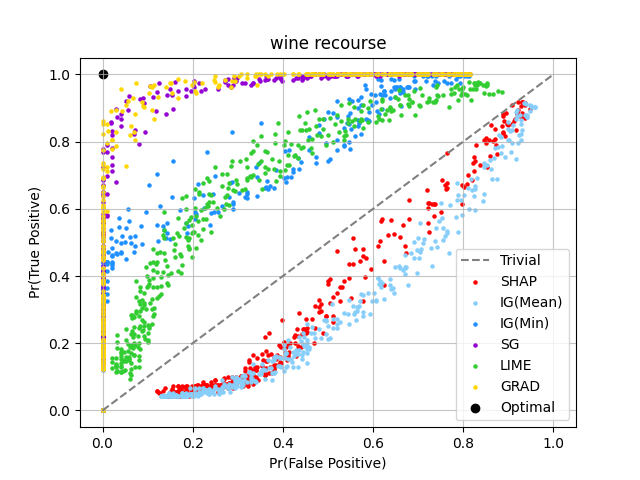
\includegraphics[width=.33\linewidth]{figure-files/experiments/10percent-plots/wine-recourse-hypothesis-tradeoff.png}
\end{subfigure}
\begin{subfigure}
    \centering
    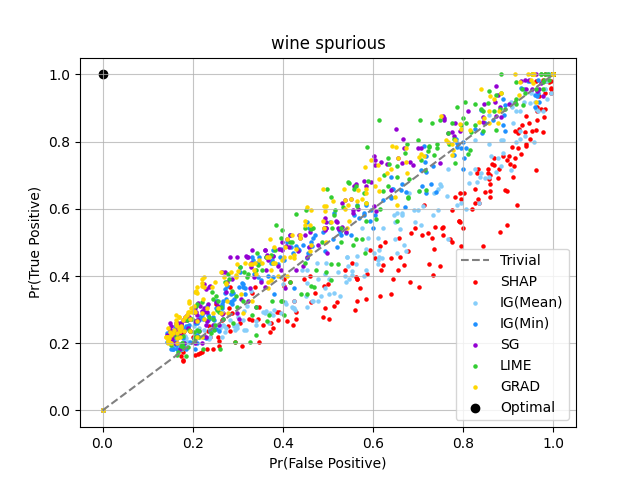
\includegraphics[width=.33\linewidth]{figure-files/experiments/10percent-plots/wine-spurious-hypothesis-tradeoff.png}
\end{subfigure}
%
%
    \caption{Visualizing ROC curves for tabular datasets. A \fielddefname{} is better for an \downtaskname{} if the ROC curve is closer to the top left corner on average.}
    \label{fig:10percent-plots-1}
\end{figure*}
\newpage

\begin{figure*}[!hpt]
\centering
%
\begin{subfigure}
    \centering
    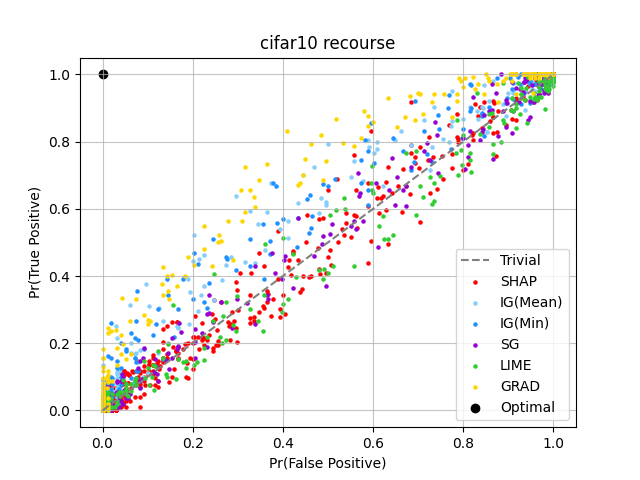
\includegraphics[width=.4\linewidth]{figure-files/experiments/10percent-plots/cifar10-recourse-hypothesis-tradeoff.png}
\end{subfigure}
\begin{subfigure}
    \centering
    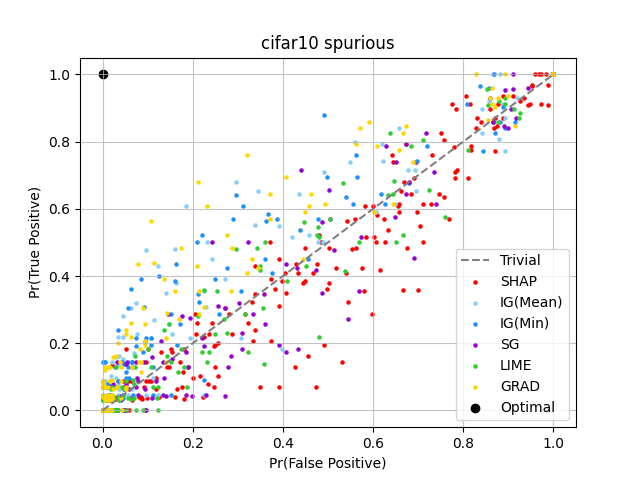
\includegraphics[width=.4\linewidth]{figure-files/experiments/10percent-plots/cifar10-spurious-hypothesis-tradeoff.png}
\end{subfigure}
%
\begin{subfigure}
    \centering
    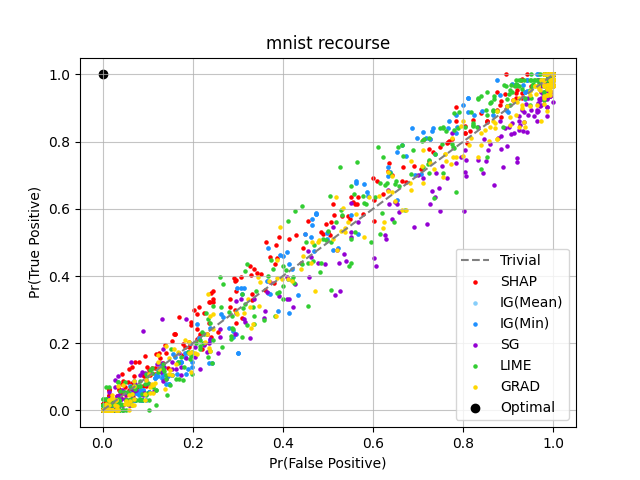
\includegraphics[width=.4\linewidth]{figure-files/experiments/10percent-plots/mnist-recourse-hypothesis-tradeoff.png}
\end{subfigure}
\begin{subfigure}
    \centering
    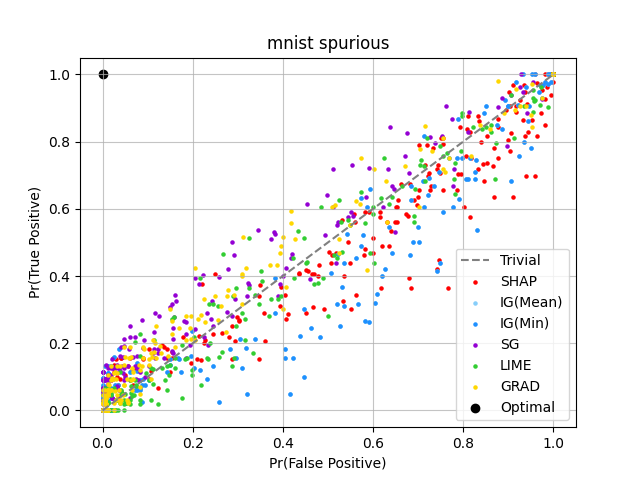
\includegraphics[width=.4\linewidth]{figure-files/experiments/10percent-plots/mnist-spurious-hypothesis-tradeoff.png}
\end{subfigure}
%
\begin{subfigure}
    \centering
    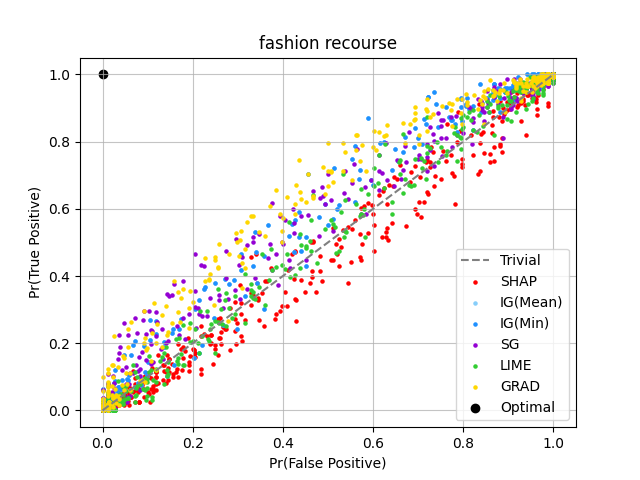
\includegraphics[width=.4\linewidth]{figure-files/experiments/10percent-plots/fashion-recourse-hypothesis-tradeoff.png}
\end{subfigure}
\begin{subfigure}
    \centering
    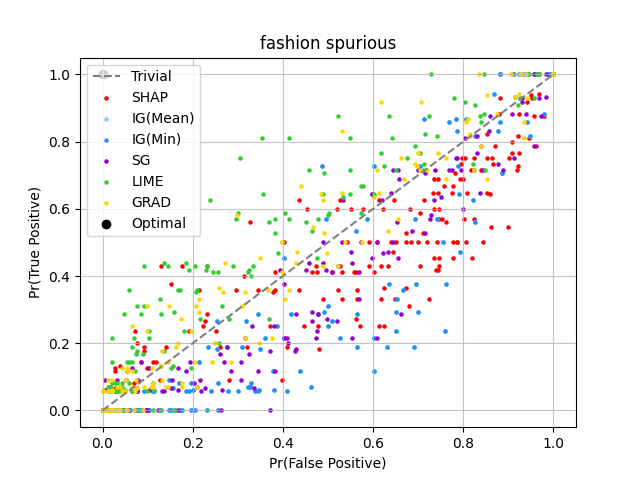
\includegraphics[width=.4\linewidth]{figure-files/experiments/10percent-plots/fashion-spurious-hypothesis-tradeoff.png}
\end{subfigure}
%
    \caption{Visualizing ROC curves for image datasets. A \fielddefname{} is better for an \downtaskname{} if the ROC curve is closer to the top left corner on average.}
    \label{fig:10percent-plots-2}
\end{figure*}
\clearpage

%
%


%
%
%
%

%
%
%

%
%
%
%
%
%
%
%
%
%
%
%
%

